\chapter{Evaluation}\label{ch:evaluation}

In this chapter we evaluate the overhead of splitting a query into multiple
multiple smaller queries using our publish/subscribe system.

\paragraph{Experimental Setup}

All experiments in this chapter were run on a dual-socket Intel Xeon E5-2650
machine (2.0GHz, 8 cores per socket, 2 threads per core) with 64 GB RAM. All components and
queries in our system were compiled with a Rust 1.14 nightly build (2016-10-20)
and executed on Debian 7.8. The input data is read from a SAN storage via
iSCSI in a private 10 Gbit ethernet.

\section{Query Composition for Sessionization}

In this experiment, we want to determine the overhead of splitting up a monolithic
dataflow computation into a dynamic set of smaller sub-queries. As data has to
be published in topics in order to be accessed by consuming queries, we expect
an increase in memory consumption and the overall execution time compared to
the case where operators copy data in-memory.

\subsection{Computation \& Workload}
The dataflow computation in this experiment is based on \emph{sessionization},
i.e. the reconstruction of user sessions from a trace of individual messages.
The input message trace is partitioned over the workers and read in parallel
through a re-order buffer.
After the sessionization, we perform a set of statistics on the reconstructed
sessions. The stages are as described below, each stage consists of a small
series of Timely operators.

\begin{description}
\item [Sessionization] Groups messages according to their session identifier.
Emits groups of messages belonging to the same session after a period of inactivity.
\item [Messages per Session] Simply counts and emits the number of messages belonging to a session.
\item [Duration of Session] Calculates the timespan between the first and last message belonging
to a session.
\item [Parse Transaction Tree] Parses the transaction identifiers for tree extraction.
\item [Transaction Tree Depth] Calculates the depth of the transaction trees.
\item [Top k Transaction Tree Signatures] Calculates signatures for the transaction trees and
reports the ten top most common tree signatures.
\item [Top k Communication Pairs] Infers the ten most common pairs of services who are
communicating with each other.
\end{description}

%It should be noted that the computational overhead of most of these stages is
%relatively low. This is shown in the cpu utilization graph.

The resulting dataflow computation is shown in Figure~\ref{fig:monolith}. For
this evaluation we split up the computation such that each stage represents
its own query. In order to achieve this, we introduce two topics: The topic
\emph{sessionize} contains the result of the sessionization stage, i.e. 
a list of messages per session. The second topic, named \emph{transactions},
is introduced for the transaction-oriented statistics. It emits a stream
containing all the transactions per session. The resulting composed dataflow
graph is shown in Figure~\ref{fig:split}, it consists of seven queries.

\begin{figure}[p]
  \centering
    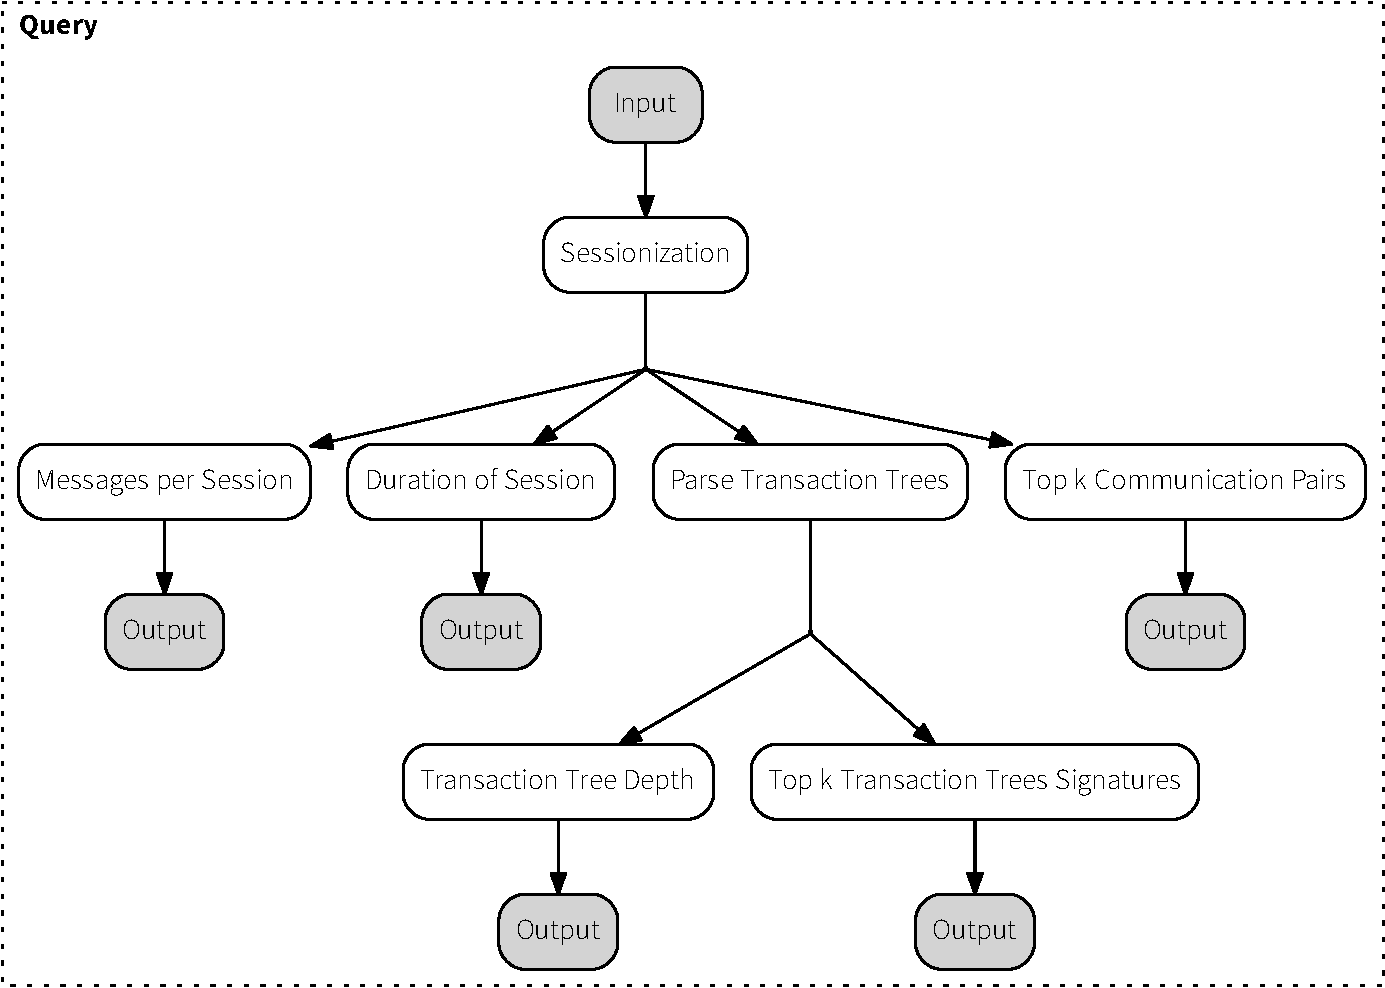
\includegraphics[width=1\textwidth]{figures/sessionize_dataflow-crop}
  \caption[Dataflow graph for monolithic sessionization]{The dataflow graph
  for the original, monolithic sessionization query.}
  \label{fig:monolith}
\end{figure}

\begin{figure}[p]
  \centering
    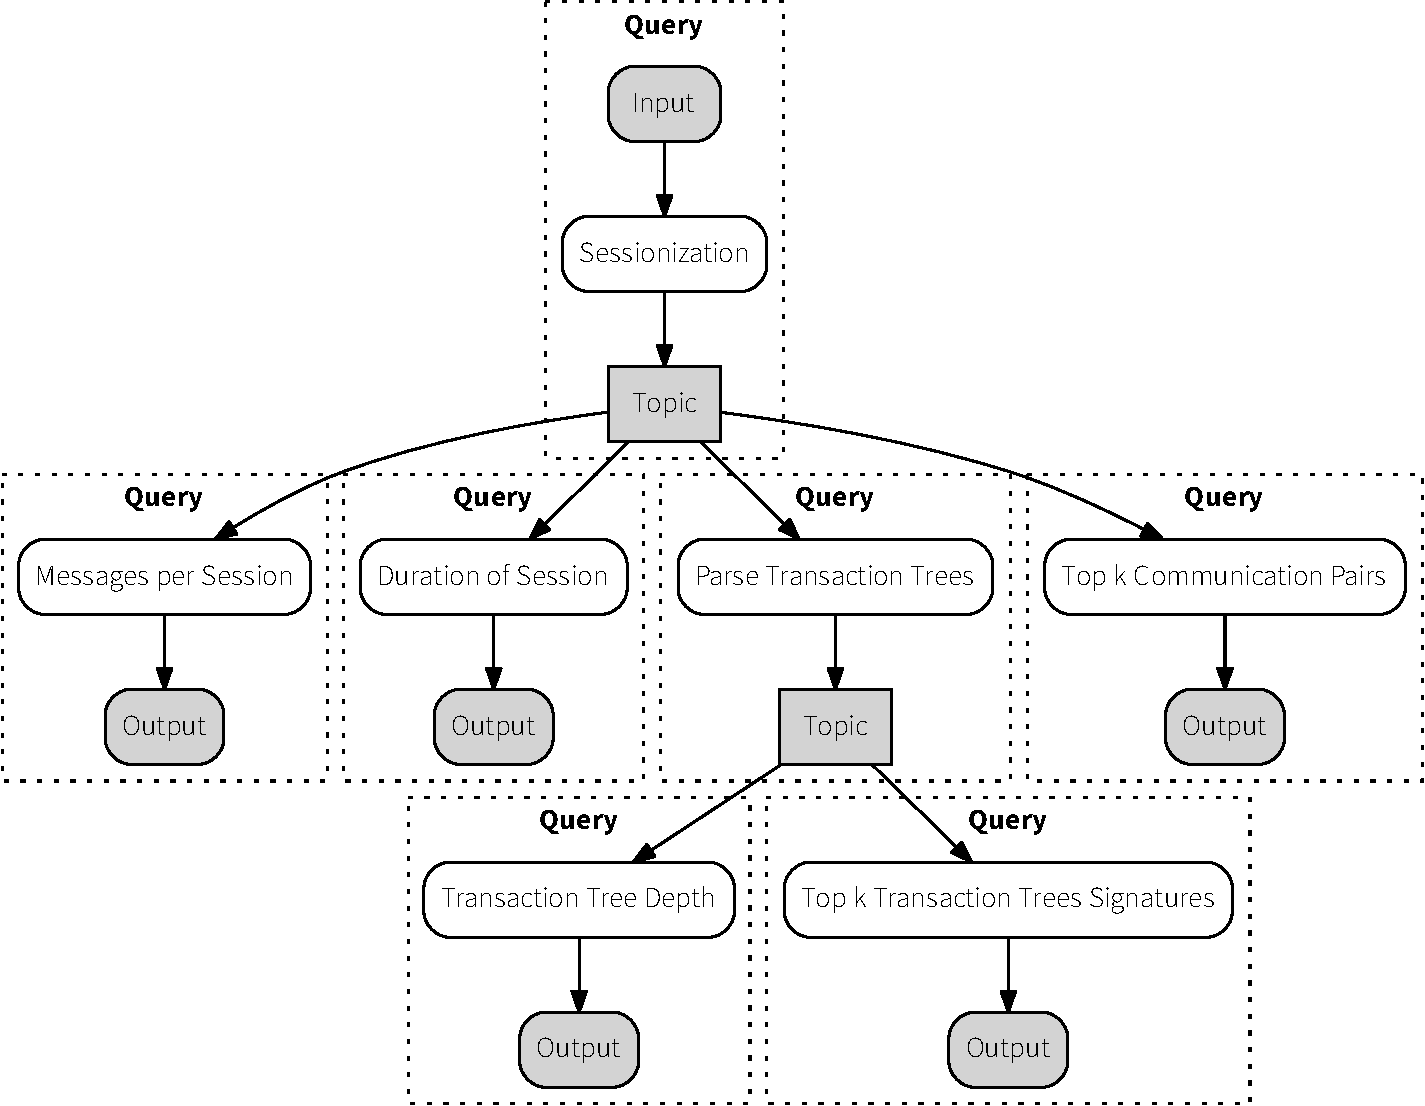
\includegraphics[width=1\textwidth]{figures/sessionize_split-crop}
  \caption[Dataflow graph for modular sessionization]{Structure of the modular
  sessionization. Two topics are introduced connect the tree of queries.}
  \label{fig:split}
\end{figure}
